\section{API}
\subsection{API Server}
\subsubsection{History of REST API}

\hspace{2cm}An API, or "application programming interface" is a set of subroutine definitions, protocols, and tools for building application software.\
 In general terms, it is a set of clearly defined methods of communication between various software components.\
 The developer creates the API on the server and allows the client to talk to it.
 
 
Prior to REST, developers used SOAP to integrate APIs. To make a call, developers handwrote an XML document with a Remote Procedure Call (RPC) call in the body. They then specified the endpoint and POST their SOAP envelope to the endpoint.
In 2000, Roy Fielding and a group of developers decided to create a standard so that any server could talk to any other server. He defined REST and the architectural constraints explained above in his 2000 PhD dissertation at UC Irvine. These universal rules make it easier for developers to integrate software.

Salesforce was the first company to sell an API as part of its “Internet as a Service” package in 2000. However, few developers were actually able to use the complicated XML API. EBay built a REST API, which expanded its market to any site that could access its API. This caught the attention of another ecommerce giant, and Amazon announced its API in 2002.

Flickr launched its own RESTful API in August 2004, enabling bloggers to easily embed images on their sites and social media feeds. Facebook and Twitter both released their APIs in 2006, buckling under the pressure of developers who scraped the sites and created “Frankenstein” APIs. When Amazon Web Services (AWS) helped launch the cloud in 2006, developers were able to access data space in minutes using AWS’s REST API, and the request for public APIs quickly escalated.
Since then, developers have embraced RESTful APIs, using them to add functionality to their websites and applications. Today, REST APIs are considered the “backbone of the Internet.”\cite{web004}
\newline \newline

\subsubsection{Work of REST API}
\hspace{2cm}REST is an architectural style that uses simple HTTP calls for inter-machine communication instead of more complex options like CORBA, COM+, RPC, or even SOAP. Using REST means your calls will be message-based and reliant on the HTTP standard to describe these messages.

Using the HTTP protocol means REST is a simple request/response mechanism. Each request returns a subsequent response. You can see what a simplified request and response look like below:
\newpage
\begin{figure}[htp]%
    \center%
    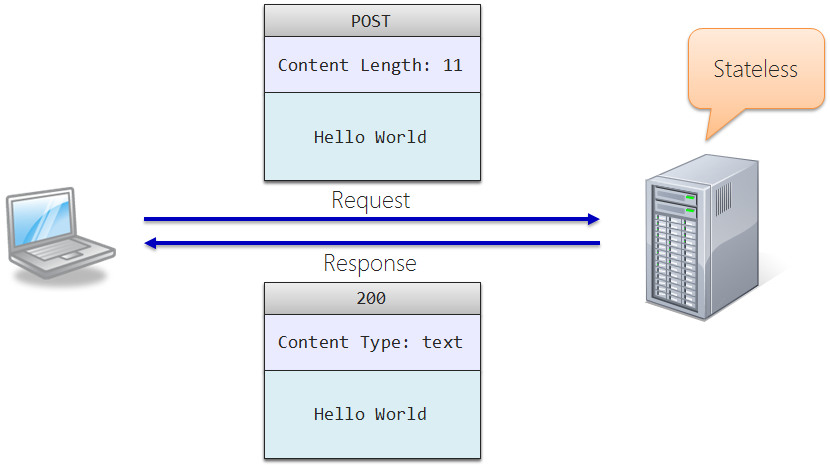
\includegraphics[width=0.8\textwidth]{images/ch4/REST-01.png}%
     % you need to add the caption for the list of figures
    \caption[Request/Response Mechanism]{Request/Response Mechanism}\label{fig: Request/Response Mechanism}%
  \end{figure}
  \newline
Requests are made up of a verb (POST, in this example), headers that describe the message, and a body (Hello World,  in this example). The request is a message that describes what you want the server to accomplish. Likewise, the response consists of three pieces: a status code (200), headers describing the response and the body itself.\newline

\textbf{HTTP Verbs describe the type of operation:}
\begin{itemize}
    \item GET: Retrieve a resource.
    \item POST: Create a resource.
    \item PUT: Update a resource.
    \item DELETE: Delete a resource.
\end{itemize}
On the Web, the most common verb is GET. This is because the main purpose of a Web page's function is to request different resources that make up a page.\\
In REST-based APIs, we leverage these verbs to describe the types of operations we want.

\subsubsection{Reasons of Using REST API}
\hspace{2cm} You could imagine that this API is accessible from a client-side Web project, an iOS app, an IoT device and even a Windows Phone. This allows you to build the infrastructure for your organization with fewer worries about the longer-term marrying to a particular client-side stack. The server lives longer than the client. It always does.

Another key idea in this architectural philosophy is that the server supports caching and is stateless. These ideas are very important to how REST works. Caching is important, as if multiple requests for the same resource are requested, caching of the result of the request means that the scalability of the server should increase.

Likewise, statelessness is about making sure that calls to the API aren't tied to a particular server, which increases the likelihood of building scalable server infrastructures. Because the server is stateless, every call to it must include all the data required to execute the request. The HTTP protocol is connectionless (there's no guarantee that your request is going to the same server, or how long it will be between those calls to the server).\cite{web005}


\subsection{Authentication and Authorization}
\hspace{2cm}In Our Project, We needed  to achieve Security so that we use authentication and authorization.\\
Authentication and authorization are both common terms in the world of identity and access management (IAM). While they might sound similar, both are distinct security processes, and understanding the difference between the two is key to successfully implementing an IAM solution.
Both authentication and authorization are required to deal with sensitive data assets. Without any of them, you are keeping data vulnerable to data breaches and unauthorized access. \\

Authentication is the act of validating that users are who they claim to be. Passwords are the most common authentication factor—if a user enters the correct password, the system assumes the identity is valid and grants access.\\
Other technologies such as One-Time Pins, authentication apps, and even biometrics can also be used to authenticate identity. In some instances, systems require the successful verification of more than one factor before granting access. This multi-factor authentication (MFA) requirement is often deployed to increase security beyond what passwords alone can provide.\\

Every organization is trying to use the best authentication process to keep their data secure. There are so many authentication processes that can be used to validate user identity.\textbf{Given below are some of them:}
\begin{itemize}
    \item Single Sign-On (SSO) allows users to get access to various applications through a single set of login credentials. SSO uses a federation when the user logs in into a spread across the different domains. 
    \item Multi-Factor Authentication (MFA) uses different means of authentication. During log in with user name and password the user is asked to provide a one-time access code that the website sends to the user’s cell phone. It provides a higher level of assurance during the authentication step to improve security.
    \item Consumer Identity and Access Management (CIAM) provides various features like customer registration, self-services account management, consent and preference management, and other authentication features.\cite{web006}
\end{itemize}

Authorization in system security is the process of giving the user permission to access a specific resource or function. This term is often used interchangeably with access control or client privilege. Giving someone permission to download a particular file on a server or providing individual users with administrative access to an application are good examples. In secure environments, authorization must always follow authentication—users should first prove that their identities are genuine before an organization’s administrators grant them access to the requested resources.\cite{web007}

\subsection{Requests Validation}
\hspace{2cm}In Our Application, We need to verify whether values of data come from the given request are acceptable values, So we use the Validation concept to achieve that.
Validation can mean a lot of things, but in API land it generally means figuring out if the data being sent to the API is any good or not.\\
\textbf{For the standard application we can put data validation logic in three places:}
 \begin{itemize}
    \item GUI – it is entry point for users input. Data is validated on the client side, for example using Javascript for web applications.
    \item Application logic/services layer – data is validated in specific application service or command handler on the server side.
    \item Database – this is exit point of request processing and last moment to validate the data.
\end{itemize}

\begin{figure}[htp]%
    \center%
    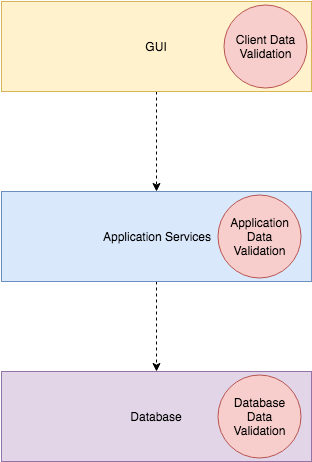
\includegraphics[width=0.6\textwidth]{images/ch4/validation.png}%
     % you need to add the caption for the list of figures
    \caption[Data validation localization]{Data validation localization}\label{fig: Data validation localization}%
  \end{figure}
\newline

Server-side validation has always been required and for an API is the most important of the two. An API that relies entirely on the client is going to end up with problems. Data coming from the client can never be trusted because it's impossible for the server to know what happened on the client. Even if you're developing a private API for only two known clients, there are always chances that validation in those clients breaks down; or someone will hit those APIs with curl or Postman and send some invalid stuff. Even if the database catches invalid data, the errors won't be useful.\\

we used Hapi Joi to achieve validation.
Hapi Joi is an object schema description language and validator for JavaScript objects.\\
Here are some very useful validation constraints that can be attached to the base schema:
\begin{itemize}
    \item allow(): Whitelists value or set of values that will always be valid before applying other rules. It can take values as its arguments or an array of values.
    \item valid(): Whitelists value or set of values as the only valid value(s) before applying other rules. It can take values as its arguments or an array of values.
    \item invalid(): Blacklists value or set of values that will never be valid. It does the direct opposite of allow(). It can take values as its arguments or an array of values.
    \item required(): Prevents the schema from allowing undefined as value.
    \item optional(): he schema can allow undefined as value. The schema however, will not allow a value of null. This is the default behaviour.
    \item raw(): This outputs the original untouched value instead of the casted value.
    \item strict(): This enables strict mode - which prevents type casting for the current key and any child keys. In non-strict mode, the values are casted to match the specified validation schema where possible. This is the default behaviour.
    \item default(): This sets a default value if the original value is undefined. In its simplest form, it takes as its first argument the value to use as default.\cite{AF0}
\end{itemize}

\subsection{Database Access}

\hspace{2cm}API handles requests & responses between a template loaded in a web browser / mobile app and a data store.
The data store can be a SQL-based database (ex: SQL Server/MySQL), or a No SQL database (ex: MongoDB), or a flat-filesystem (text/json files).\\
When a HTTP-based request is made from the API end-point (http/https URL), the software uses the data store to process the request and then returns a HTTP-based response to the web template which is then displayed in the web browser or the mobile app.

 For Details, When a client-side  requests some data to an API, passing the filter conditions, and parameters. API goes to the database (read hits the database) with the access credentials known to it (or the shared credentials passed as parameters), fetches the records from the relevant tables in the database, wraps them and tags them, and returns to the client-side as a returning parameter or sends to an address as passed in the parameters.
 
Being a server-side code the API uses the data store connection option / library available to the programming language in which it is written.


\subsection{APIs Integrations}

\hspace{2cm}The term API integration refers to how two or more applications can be connected via their APIs to perform some joint function or to have the results which we need..using the API layer of two or more applications to make them talk to each other.\\
We need to integrate with other APIs to use their services and functions in our project to be more performance and efficiency.\\
For Example, we need to define locations through GPS so we integrated with Google Maps API to do this process.\\
Another Example, we need to manage debit and credit cards to make online Payment available in our application so we use Stripe to achieve this.\\

\textbf{Below are the  APIs which we used:}\\
-Google Maps APIs:

\hspace{1cm}--Distance API: to measure distances.

\hspace{1cm}--Directions API: define directions of movement.

\hspace{1cm}--Places API: get locations names and details.

-Firebase Cloud Messaging(FCM): to push notification.

-Stripe: to Manage debit and credit cards.

-Paypal: manage paypal banking accounts.

-SendGrid: send mails.

-Nexmo: send sms.



\subsection{ Handling and Logging Error}
\hspace{2cm}Our application don’t run in an ideal world. Unexpected errors can happen as a result of bugs in our code or issues in the running environment.\\
For example, our MongoDB server may shut down, or a remote HTTP service we call may go down.\\
As a good developer, you should count for these unexpected errors, log them, and return a proper error to the client in a message.\\
- Use the Express error middleware to catch any unhandled exceptions in the “request processing pipeline”.\\
- To pass control to the error middleware, wrap your route handler code in a try/catch block and call next().\\
- Adding a try/catch block to every route handler is repetitive and time consuming So Using express-async-errors module.\\
This module will monkey-patch your route handlers at runtime. It’ll wrap your code within a try/catch block and pass unhandled errors to your error middleware.\\
- To log errors use winston.\\
- Winston can log errors in multiple transports. A transport is where your log is stored.\\
The error middleware in Express only catches exceptions in the request
processing pipeline. Any errors happening during the application startup (eg connecting to MongoDB) will be invisible to Express.\\
- Use process.on(‘uncaughtException’) to catch unhandled exceptions, and
process.on(‘unhandledRejection’) to catch rejected promises.\cite{AF1}



















 
 